\chapter{อุปกรณ์ต้นแบบและการแสดงผลบนหน้าจอ}



\section{รูปอุปกรณ์ที่ใช้ในการตรวจจับภาพใบหน้าและรับคำสั่งยืนยัน}

% Text for a section in the first appendix goes here.

% test ทดสอบฟอนต์ serif ภาษาไทย
\begin{figure}[!ht]
  \begin{center}
    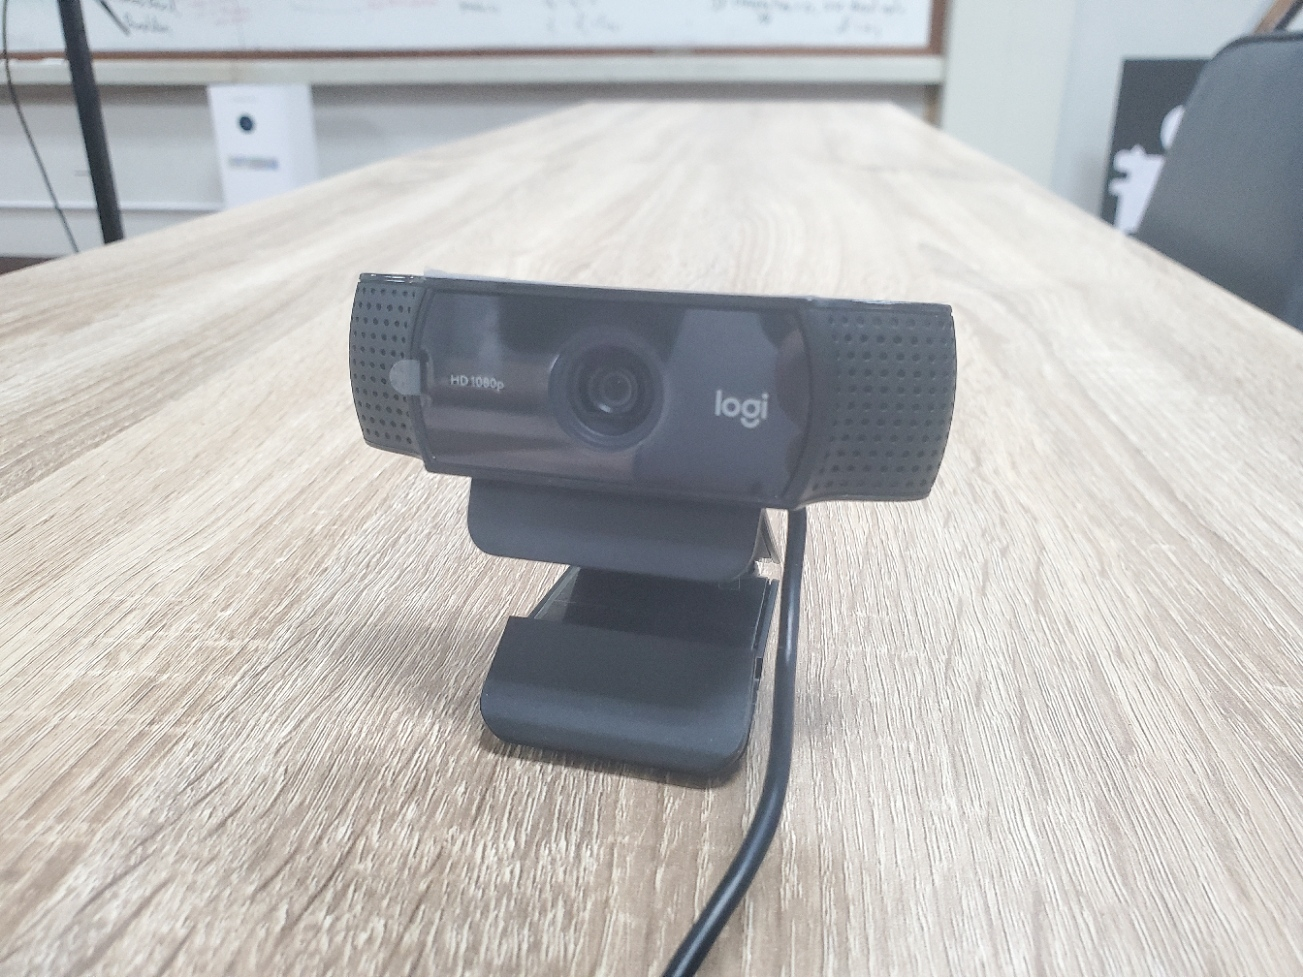
\includegraphics[scale=.2]{pic/camera.jpg}
    \caption[camera]{กล้องที่ใช้ในการตรวจจับใบหน้าบุคคล}
    \label{fig:camera_logi}
  \end{center}
\end{figure}

\begin{figure}[!ht]
  \begin{center}
    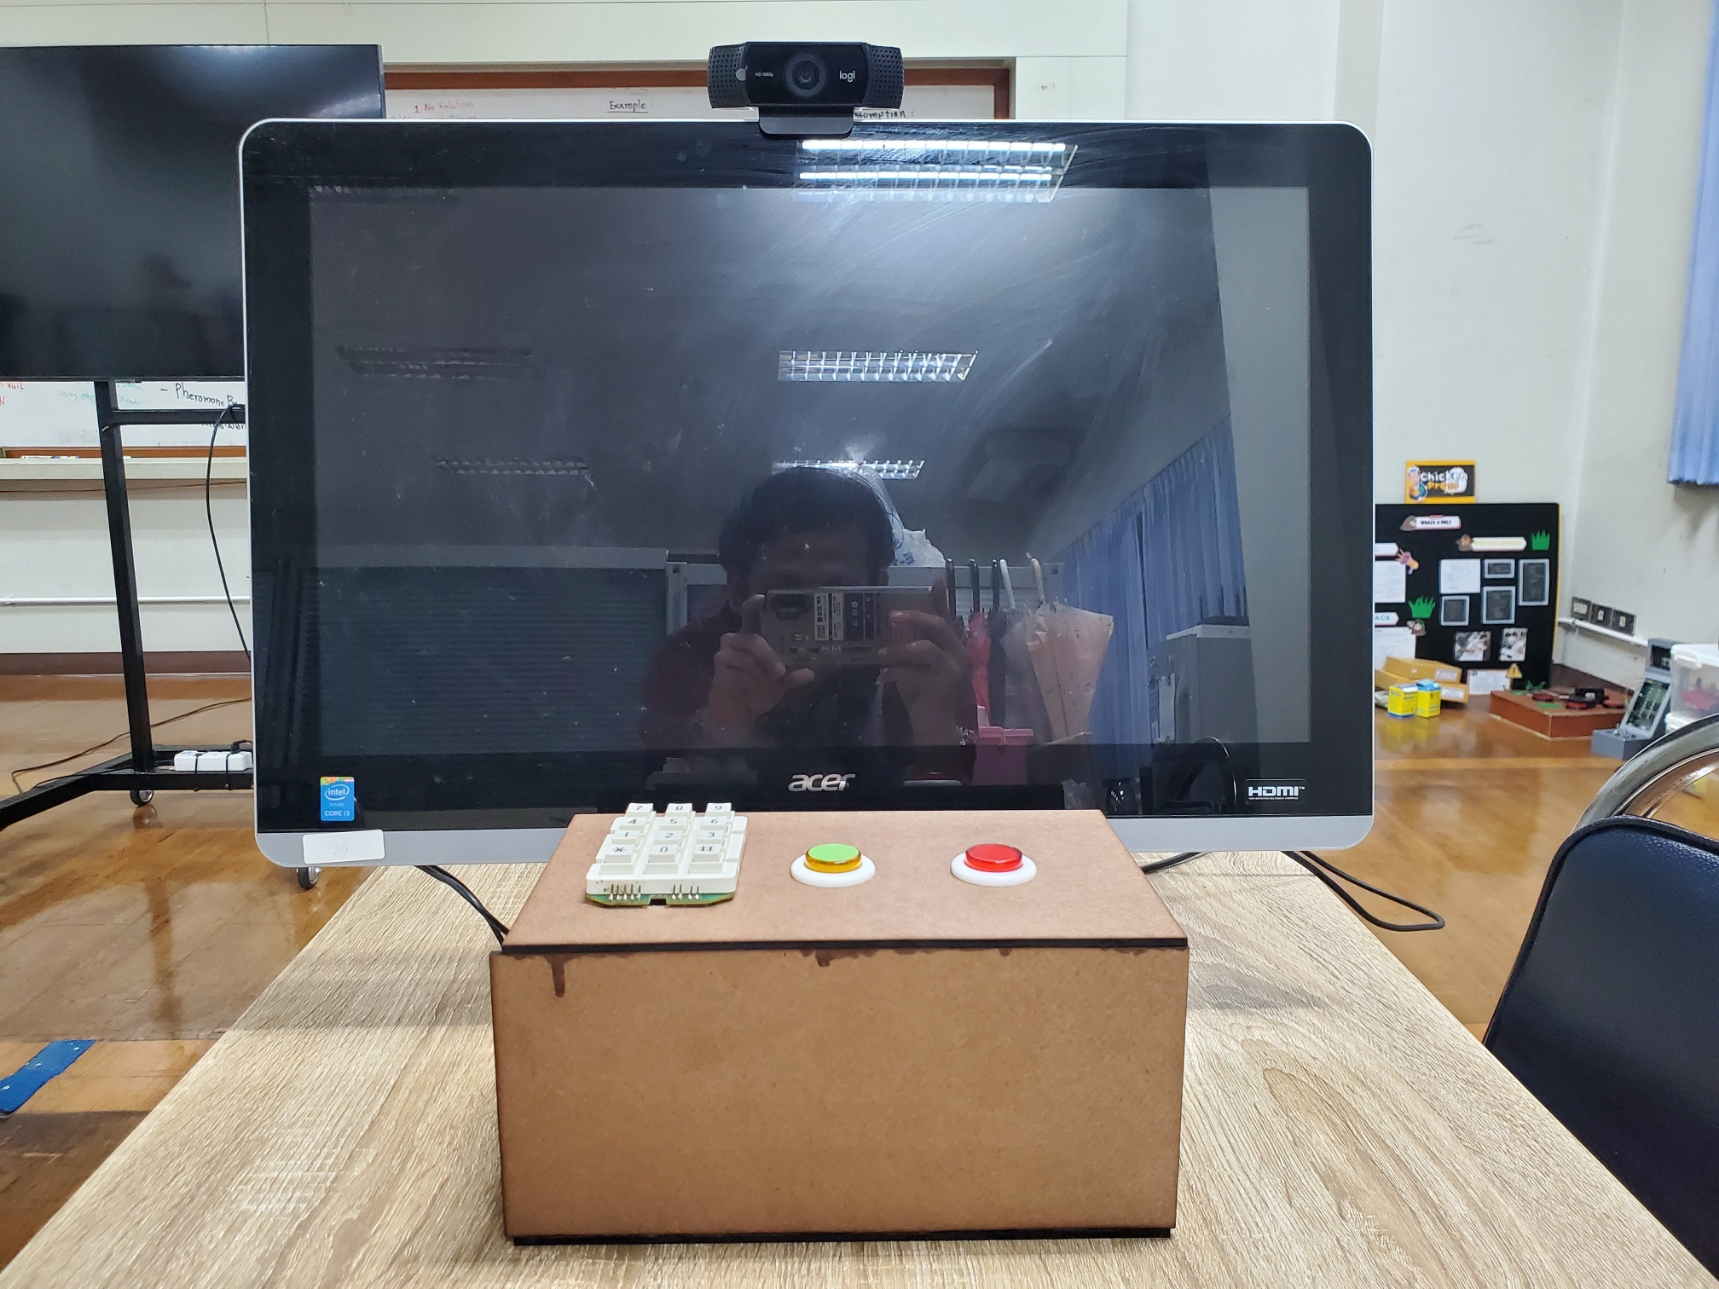
\includegraphics[scale=.2]{pic/system.jpg}
    \caption[face detection module]{มอดูลที่ใช้ในการระบุตัวตนด้วยรูปภาพใบหน้าและแสดงผล}
    \label{fig:face_module}
  \end{center}
\end{figure}

\begin{figure}[!ht]
  \begin{center}
    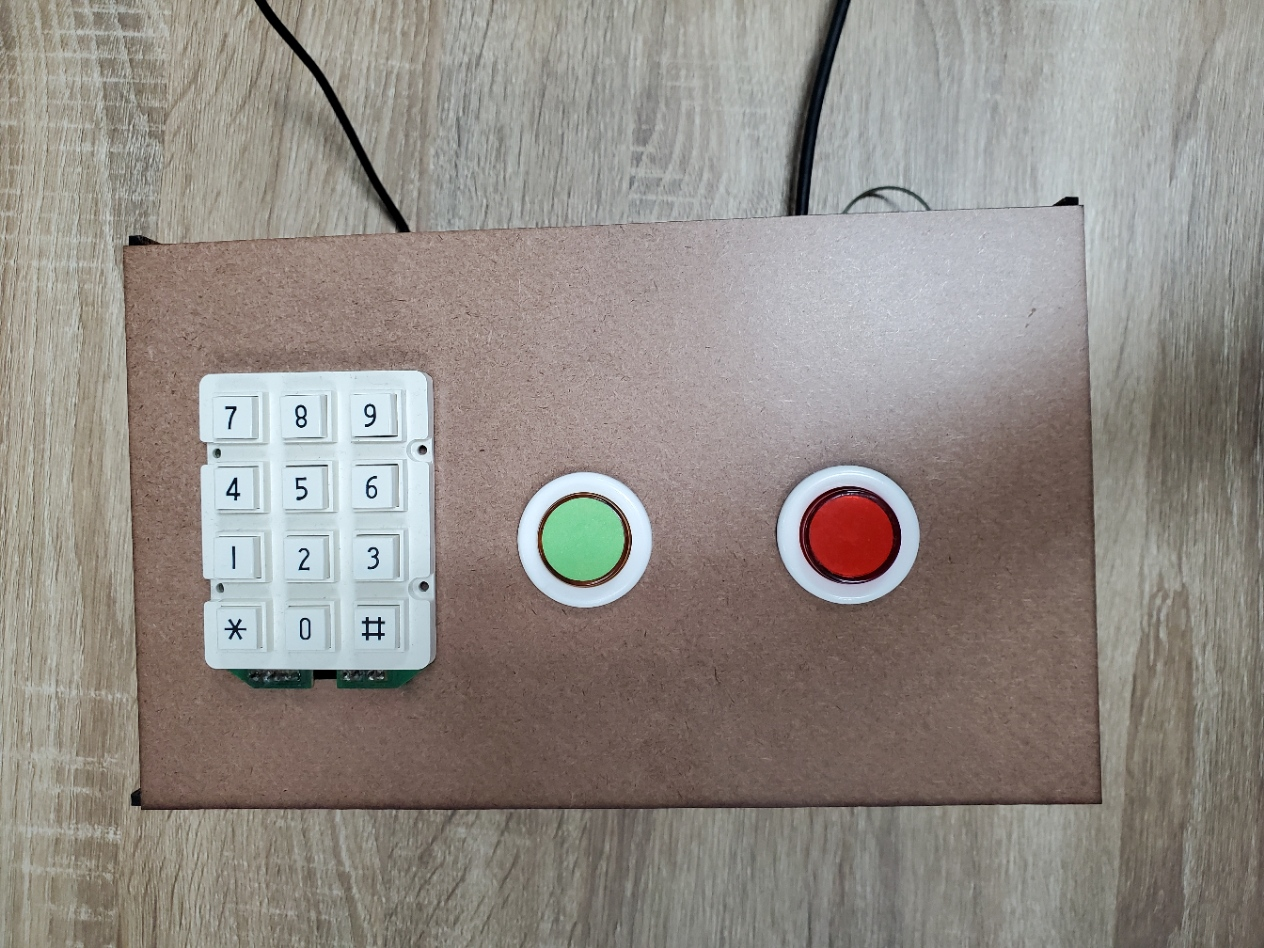
\includegraphics[scale=.2]{pic/rpi_top.jpg}
    \caption[button]{ปุ่มกดให้คะแนนความถูกต้อง}
    \label{fig:button_module}
  \end{center}
\end{figure}

\begin{figure}[!ht]
  \begin{center}
    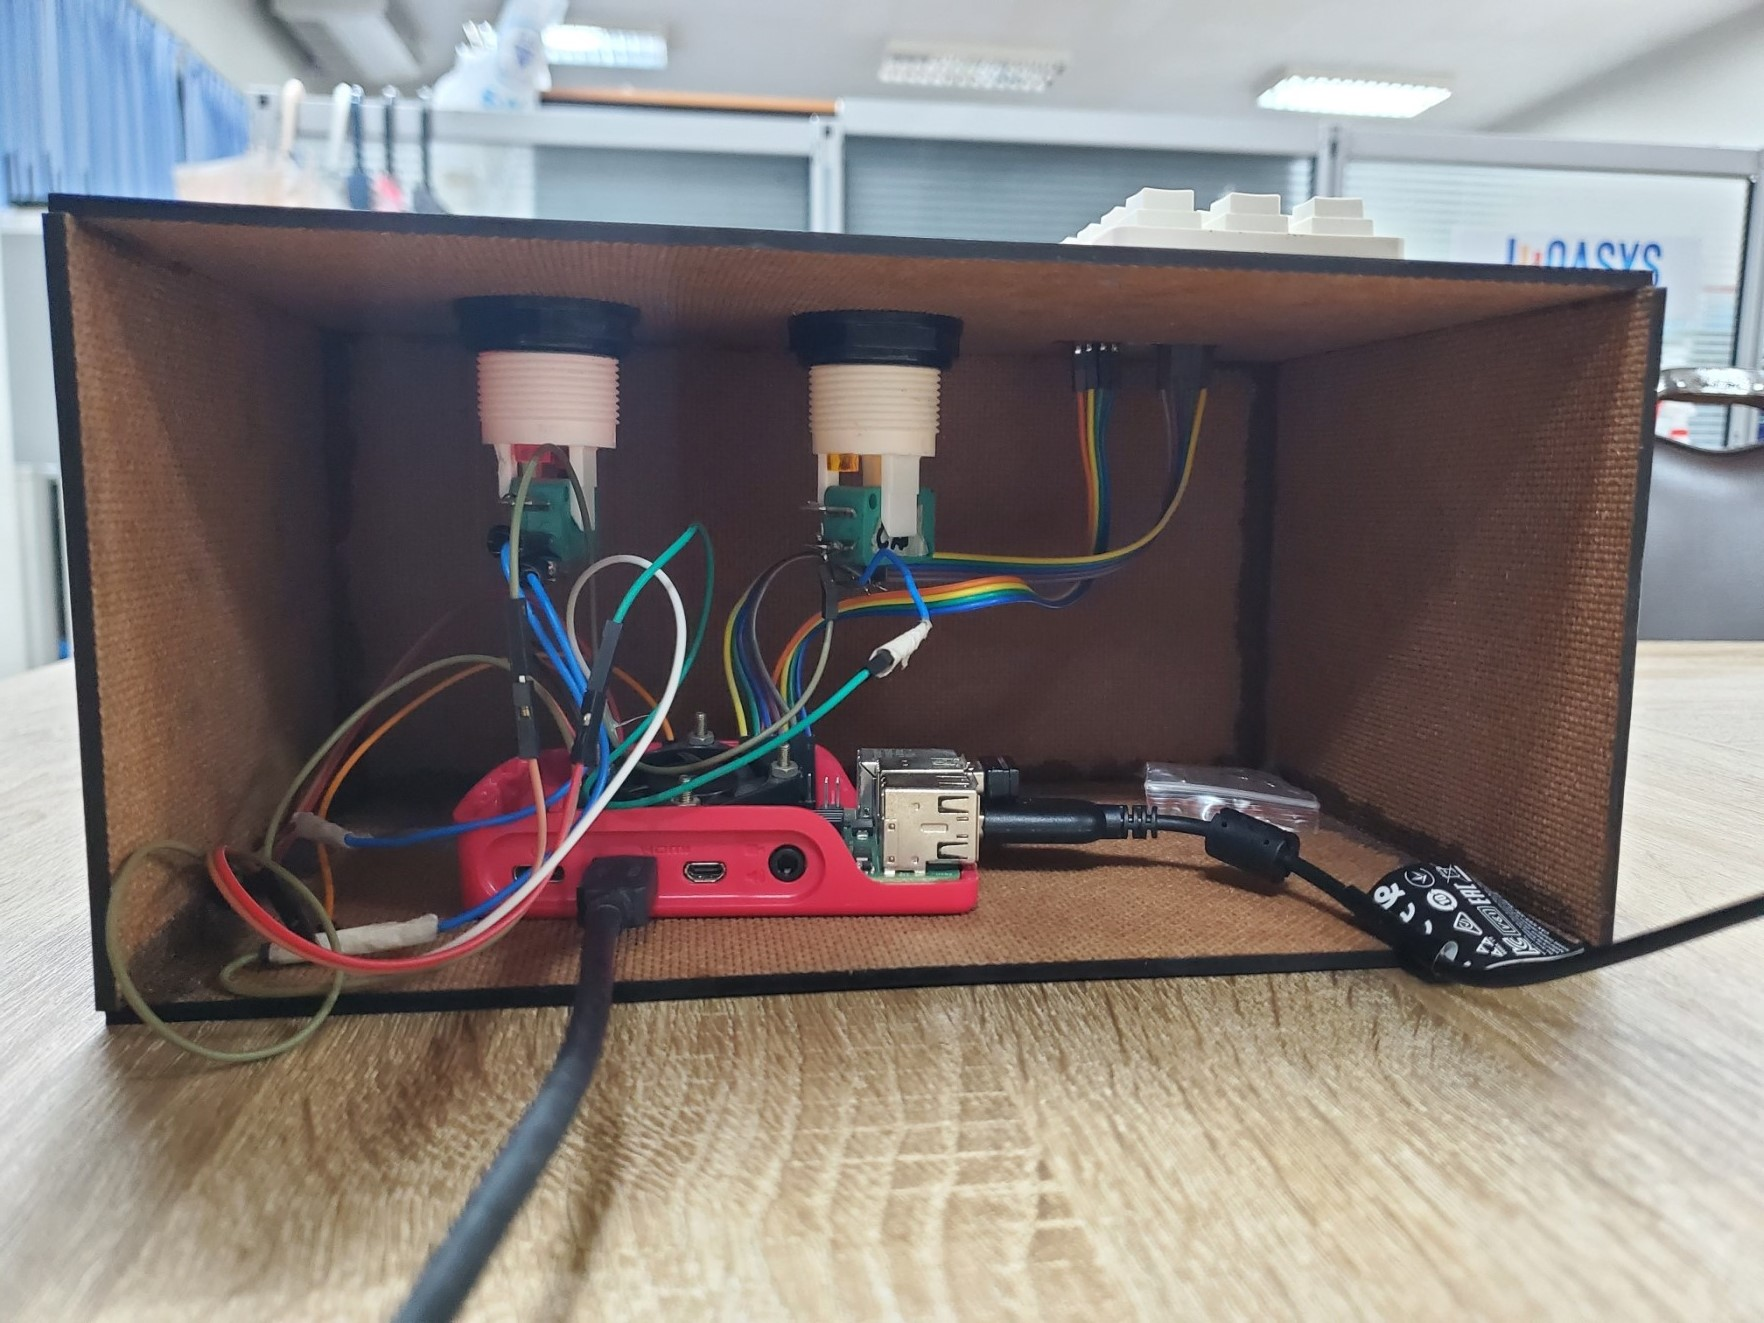
\includegraphics[scale=.2]{pic/rpi_back.jpg}
    \caption[inside module]{แสดงภายในมอดูลการตรวจจับใบหน้าและแสดงผล}
    \label{fig:inside_module}
  \end{center}
\end{figure}

\begin{figure}[!ht]
  \begin{center}
    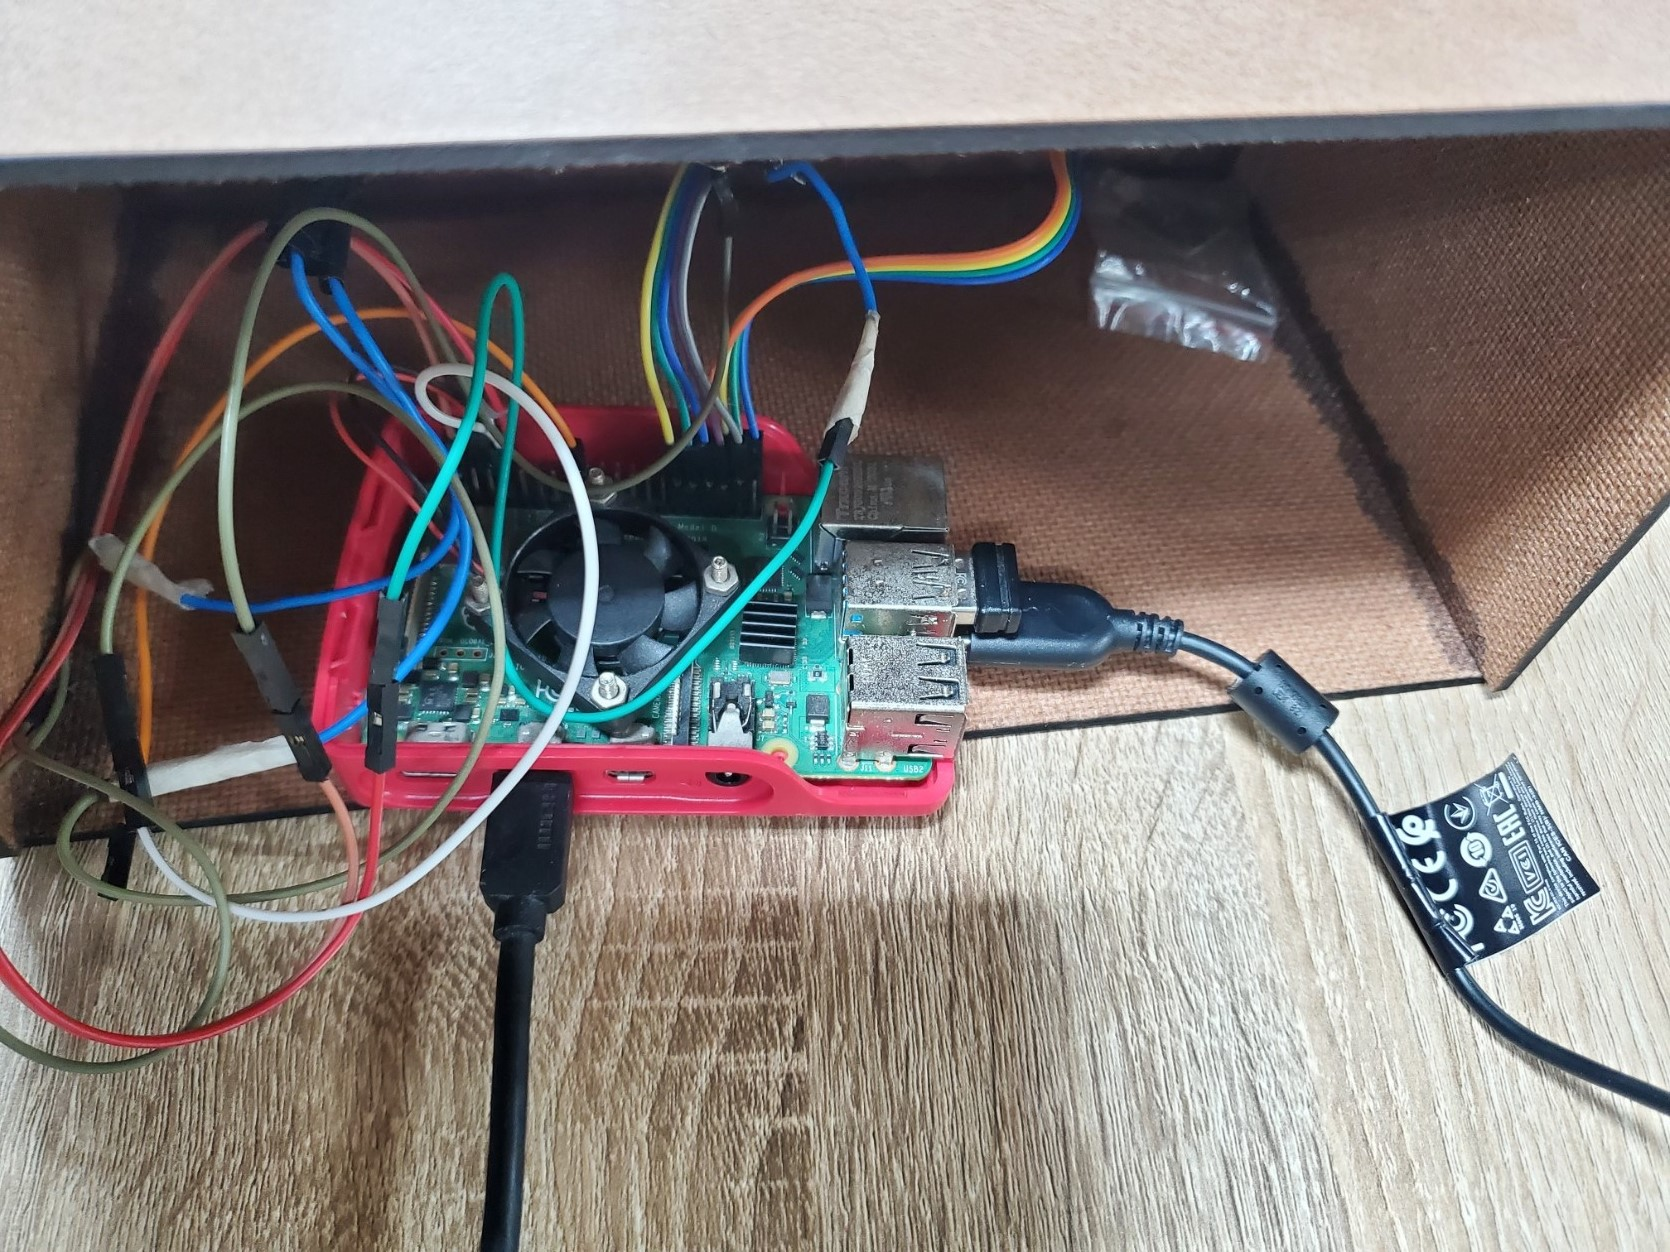
\includegraphics[scale=.2]{pic/rpi.jpg}
    \caption[Raspberry Pi]{แสดงการเชื่อมต่อ Raspberry Pi}
    \label{fig:rpi_module}
  \end{center}
\end{figure}


\section{รูปภาพการแสดงผลบนหน้าจอ}

\begin{figure}[!ht]
    \begin{center}
      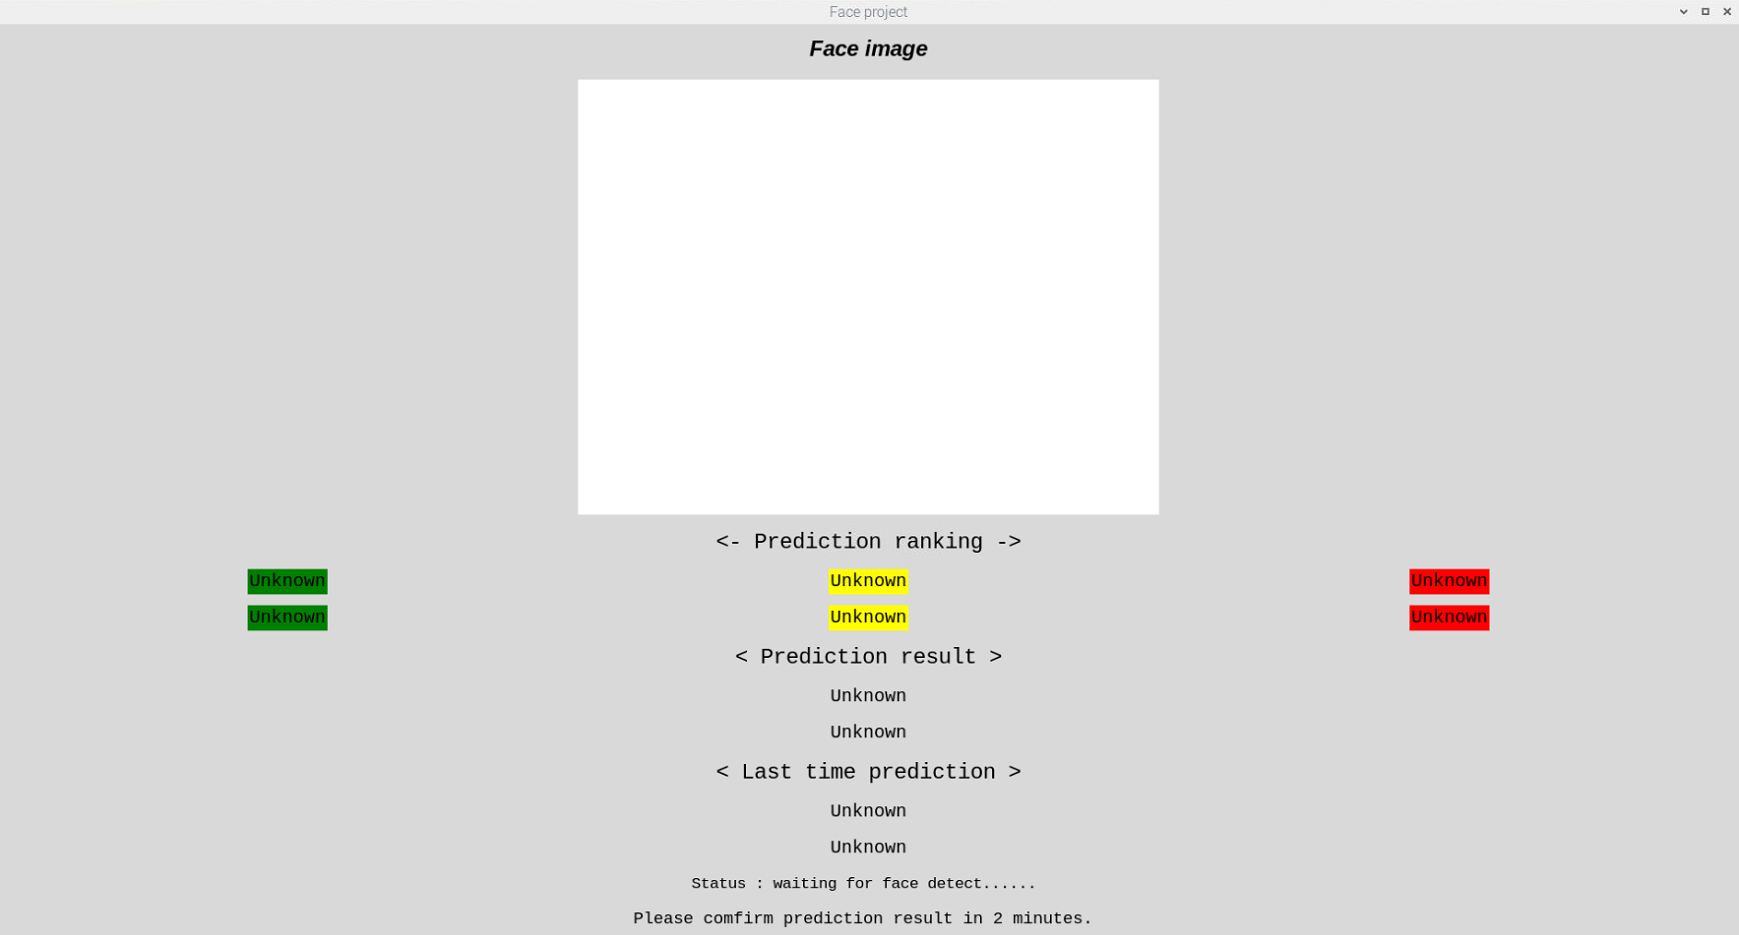
\includegraphics[scale=.4]{pic/main_page.png}
      \caption[main page]{แสดงหน้า GUI เมื่อโปรแกรมเริ่มทำงาน}
      \label{fig:main_page}
    \end{center}
  \end{figure}



\begin{figure}[!ht]
    \begin{center}
      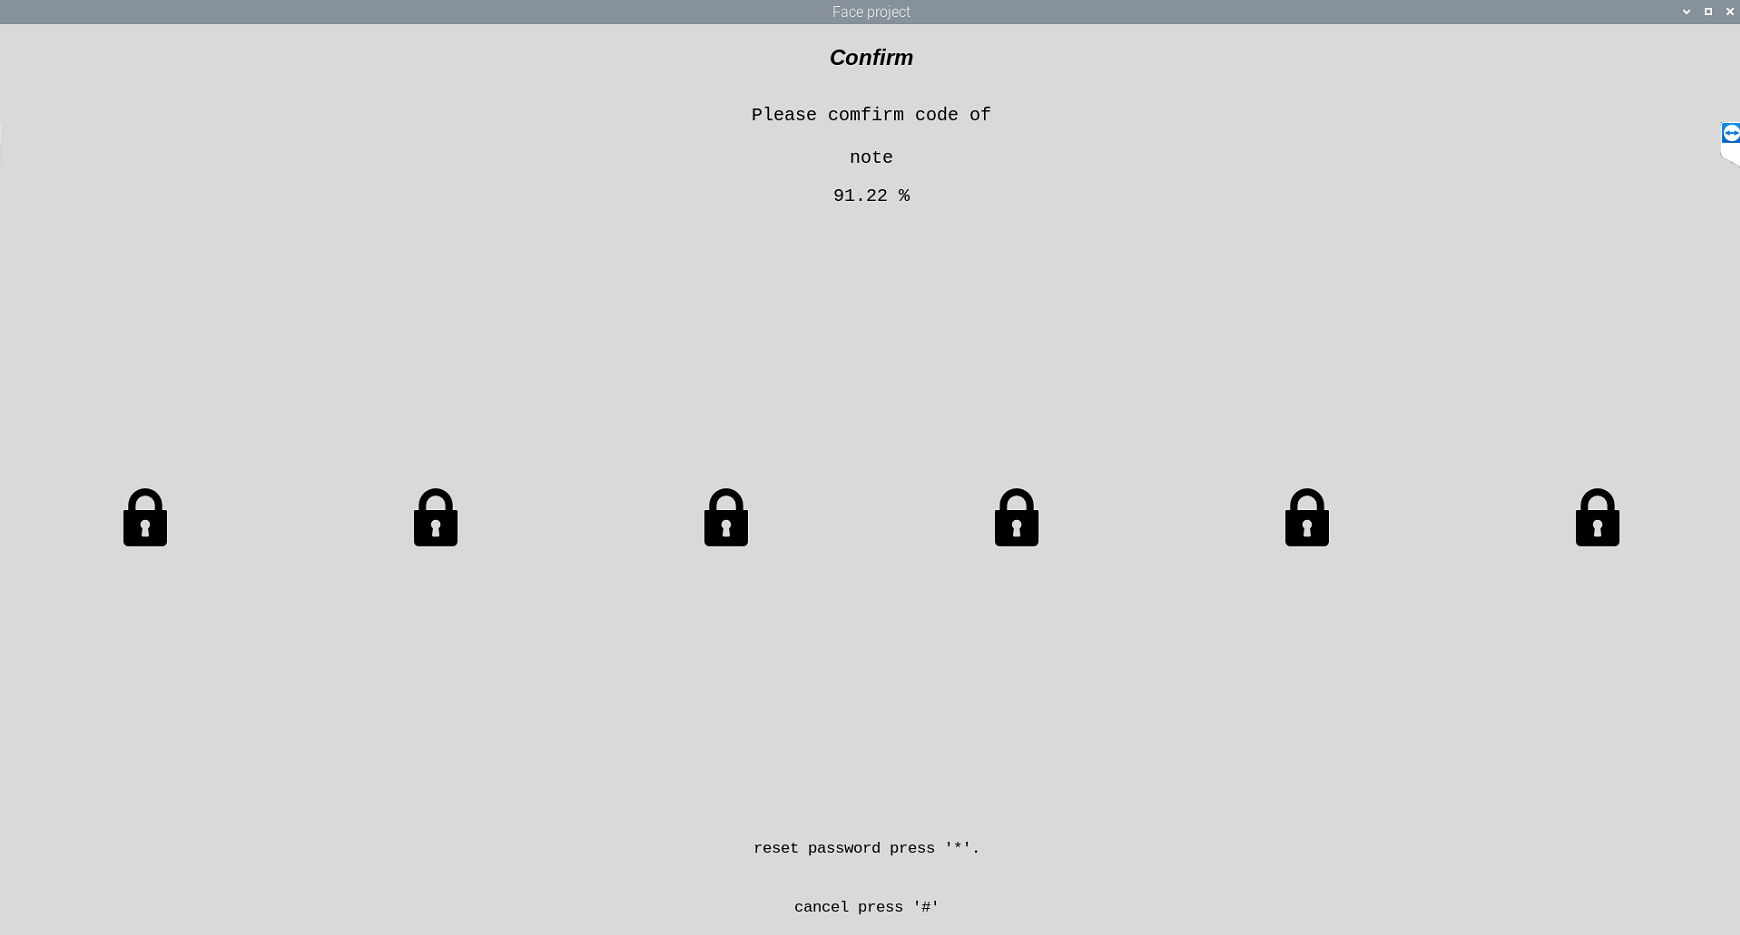
\includegraphics[scale=.4]{pic/comfirm_page.png}
      \caption[wrong predict]{แสดงหน้า GUI เมื่อผลลัพธ์การระบุตัวตนผิด}
      \label{fig:com_page}
    \end{center}
  \end{figure}



\newpage

\textsf{test ทดสอบฟอนต์ sans serif ภาษาไทย}

\verb+test ทดสอบฟอนต์ teletype ภาษาไทย+

\texttt{test ทดสอบฟอนต์ teletype ภาษาไทย}

\textbf{ตัวหนา serif ภาษาไทย \textsf{sans serif ภาษาไทย} \texttt{teletype ภาษาไทย}}

\textit{ตัวเอียง serif ภาษาไทย \textsf{sans serif ภาษาไทย} \texttt{teletype ภาษาไทย}}

\textbf{\textit{ตัวหนาเอียง serif ภาษาไทย \textsf{sans serif ภาษาไทย} \texttt{teletype ภาษาไทย}}}






\chapter{\ifenglish Manual\else คู่มือการใช้งานระบบ\fi}

โปรแกรมของโครงงานนี้สามารถดาวน์โหลดได้จาก \url{https://www.example.com/test_ทดสอบ_url} 
และใช้ระบบปฏิบัติการ Raspberry Pi คือ Raspbian buster

\section{คู่มือการติดตั้ง OpenCV บน Raspberry Pi}
\begin{enumerate}
  \item เปิด Termenal
  \item พิมพ์คำสั่ง sudo git clone https://github.com/freedomwebtech/raspbianlegacy.git
  \item พิมพ์คำสั่ง cd raspbianlegacy
  \item พิมพ์คำสั่ง sudo chmod 775 install.sh
  \item พิมพ์คำสั่ง sudo ./install.sh จากนั้นรอจนกว่าจะเสร็จ ใช้เวลาประมาณ 2 ชั่วโมง
  \item เมื่อทำการติดตั้งเสร็จแล้วให้ทดลองใช้คำสั่ง python3
  \item แล้วพิมพ์ import cv2
  \item แล้วพิมพ์ cv2.\textunderscore\textunderscore version \textunderscore\textunderscore
\end{enumerate}

\section{คู่มือการติดตั้ง TensorFlow lite บน Raspberry Pi}
\begin{enumerate}
  \item เปิด Termenal
  \item พิมพ์คำสั่ง sudo git clone https://github.com/freedomwebtech/raspbianlegacy.git
  \item พิมพ์คำสั่ง cd raspbianlegacy
  \item พิมพ์คำสั่ง sudo chmod 775 tensorflow-lite.sh
  \item พิมพ์คำสั่ง sudo ./tensorflow-lite.sh จากนั้นรอจนกว่าจะเสร็จ
  \item เมื่อทำการติดตั้งเสร็จแล้วให้ทดลองใช้คำสั่ง pip show tensorflow หากติดตั้งสำเร็จจะขึ้นข้อมูลของ tensorflow
\end{enumerate}

\section{คู่มือการติดตั้ง TensorFlow lite บน Raspberry Pi}
\begin{enumerate}
  \item เปิด Termenal
  \item พิมพ์คำสั่ง sudo apt update
  \item พิมพ์คำสั่ง sudo pip3 install mediapipe-rpi4 จากนั้นรอจนกว่าจะเสร็จ
\end{enumerate}

\section{คู่มือการใช้งานอุปกรณ์ในการตรวจจับใบหน้า}



\section{คู่มือการใช้งานอุปกรณ์ในการตรวจจับใบหน้า}
